\begin{wrapfigure}[2]{r}[-1cm]{4cm}
 \vspace{-6cm}
  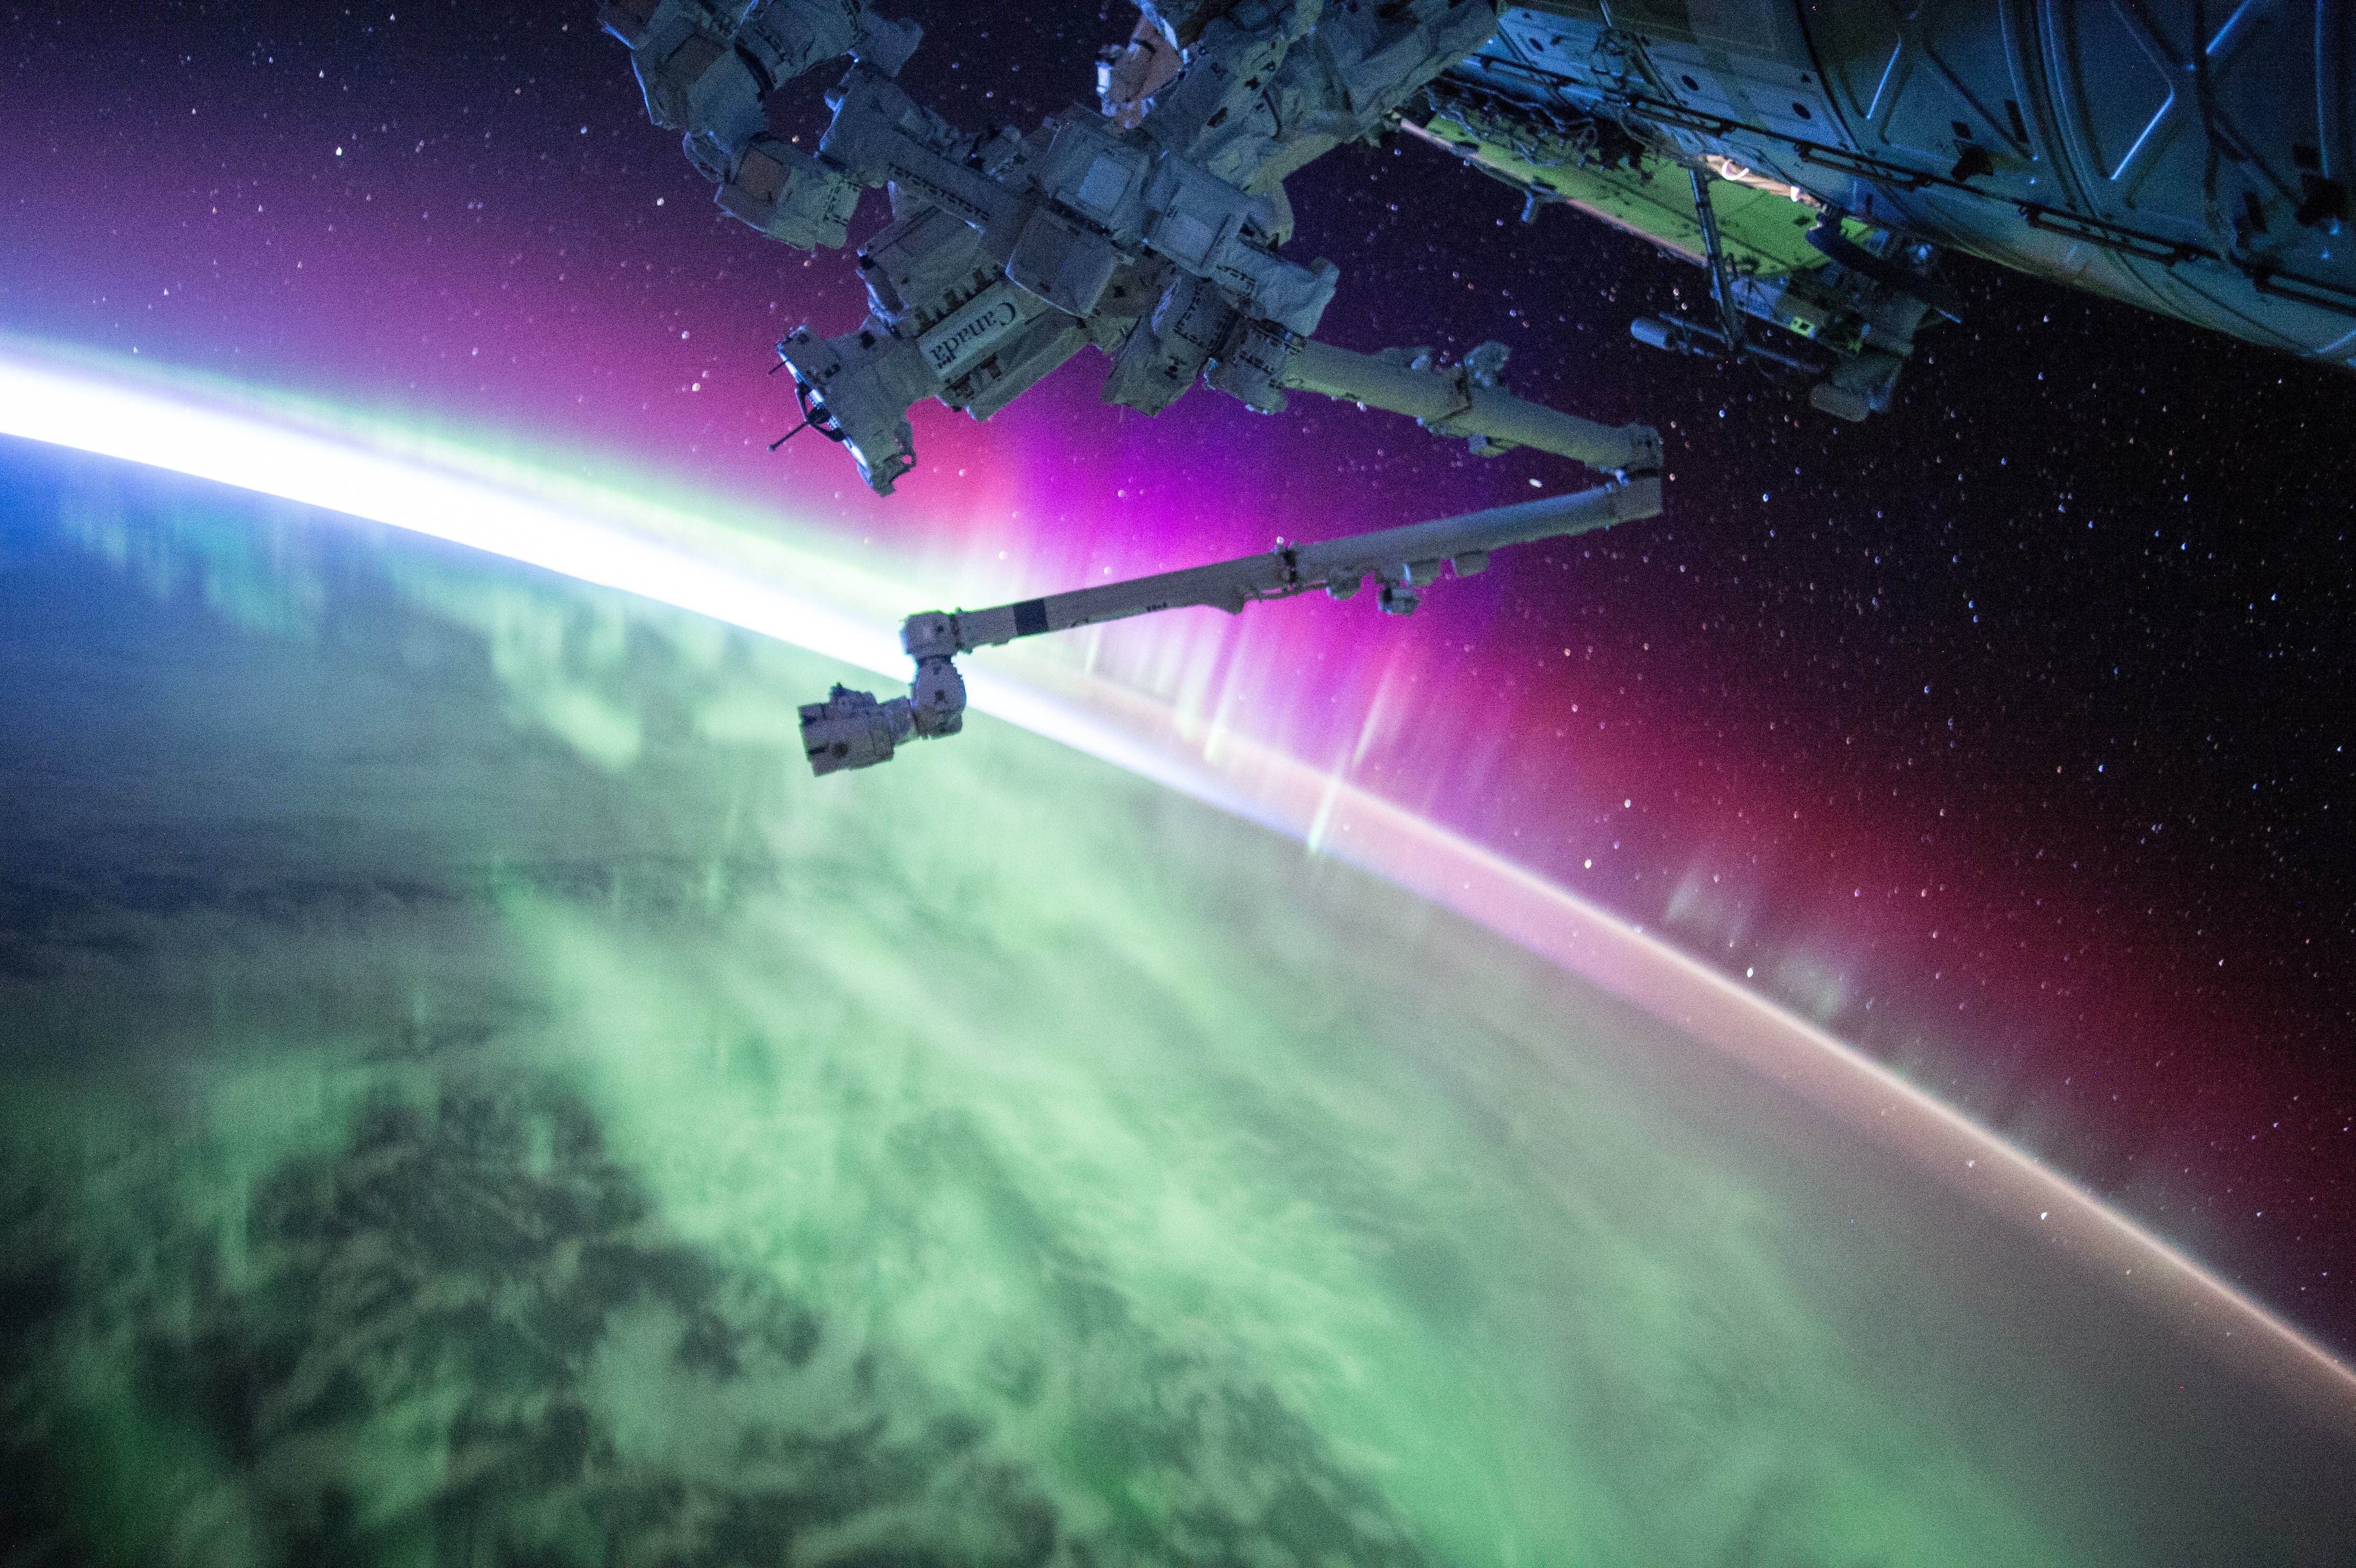
\includegraphics[scale=0.04]{Wellenausbreitung/Bilder/aurora.jpeg}
 \vspace{-6cm}
\end{wrapfigure}

\section{Theorie- und Prüfungsfragen}

~~~~~~
\subsection*{Kurzwellenausbreitung}

\begin{enumerate} 
\itemsep1pt\parskip0pt\parsep0pt
\item[1] \emph{\textbf{TI203}}  Welche der folgenden Aussagen trifft für KW-Funkverbindungen zu, die über Bodenwellen erfolgen? Die Bodenwelle folgt der Erdkrümmung und ...
	\begin{enumerate}
	\itemsep1pt\parskip0pt\parsep0pt
		\item[A] geht nicht über den geografischen Horizont hinaus. Sie wird in höheren Frequenzbereichen stärker gedämpft als in niedrigeren Frequenzbereichen.
		\item[B] geht über den geografischen Horizont hinaus. Sie wird in niedrigeren Frequenzbereichen stärker gedämpft als in höheren Frequenzbereichen.
		\item[C] geht über den geografischen Horizont hinaus. Sie wird in höheren Frequenzbereichen stärker gedämpft als in niedrigeren Frequenzbereichen.
		\item[D] geht nicht über den geografischen Horizont hinaus. Sie wird in niedrigeren Frequenzbereichen stärker gedämpft als in höheren Frequenzbereichen.
	\end{enumerate}
\loesung{Lösung C}
\end{enumerate}

\subsection*{Ionosphäre}

\begin{enumerate} 
\itemsep1pt\parskip0pt\parsep0pt
\item[2] \emph{\textbf{TI103}}  In welcher Höhe befinden sich die für die Fernausbreitung (DX) wichtigen ionosphärischen Schichten? Sie befinden sich in ungefähr ...
	\begin{enumerate}
	\itemsep1pt\parskip0pt\parsep0pt
		\item[A] 2 bis 5 km Höhe.
		\item[B] 20 bis 50 km Höhe.
		\item[C] 200 bis 500 km Höhe.
		\item[D] 2000 bis 5000 km Höhe.
	\end{enumerate}
\loesung{Lösung C}
\end{enumerate}

\begin{enumerate} 
\itemsep1pt\parskip0pt\parsep0pt
\item[3] Ergänze folgendes Schaubild: Abbildung  \ref{welle}. Tragen Sie die Bezeichnungen der einzelnen Schichten ein, die Höhe in der sie sich etwa befindet und die wichtigsten Frequenzen.
\end{enumerate}

\begin{figure}[H]
\def\svgwidth{\columnwidth}
\input{Wellenausbreitung/Bilder/Wellenausbreitung2.pdf_tex}
\label{welle}
\end{figure}

\loesung{
\begin{figure}[H]
\def\svgwidth{\columnwidth}
\begin{wrapfigure}[0]{r}[-1cm]{4cm}
 \vspace{-6cm}
  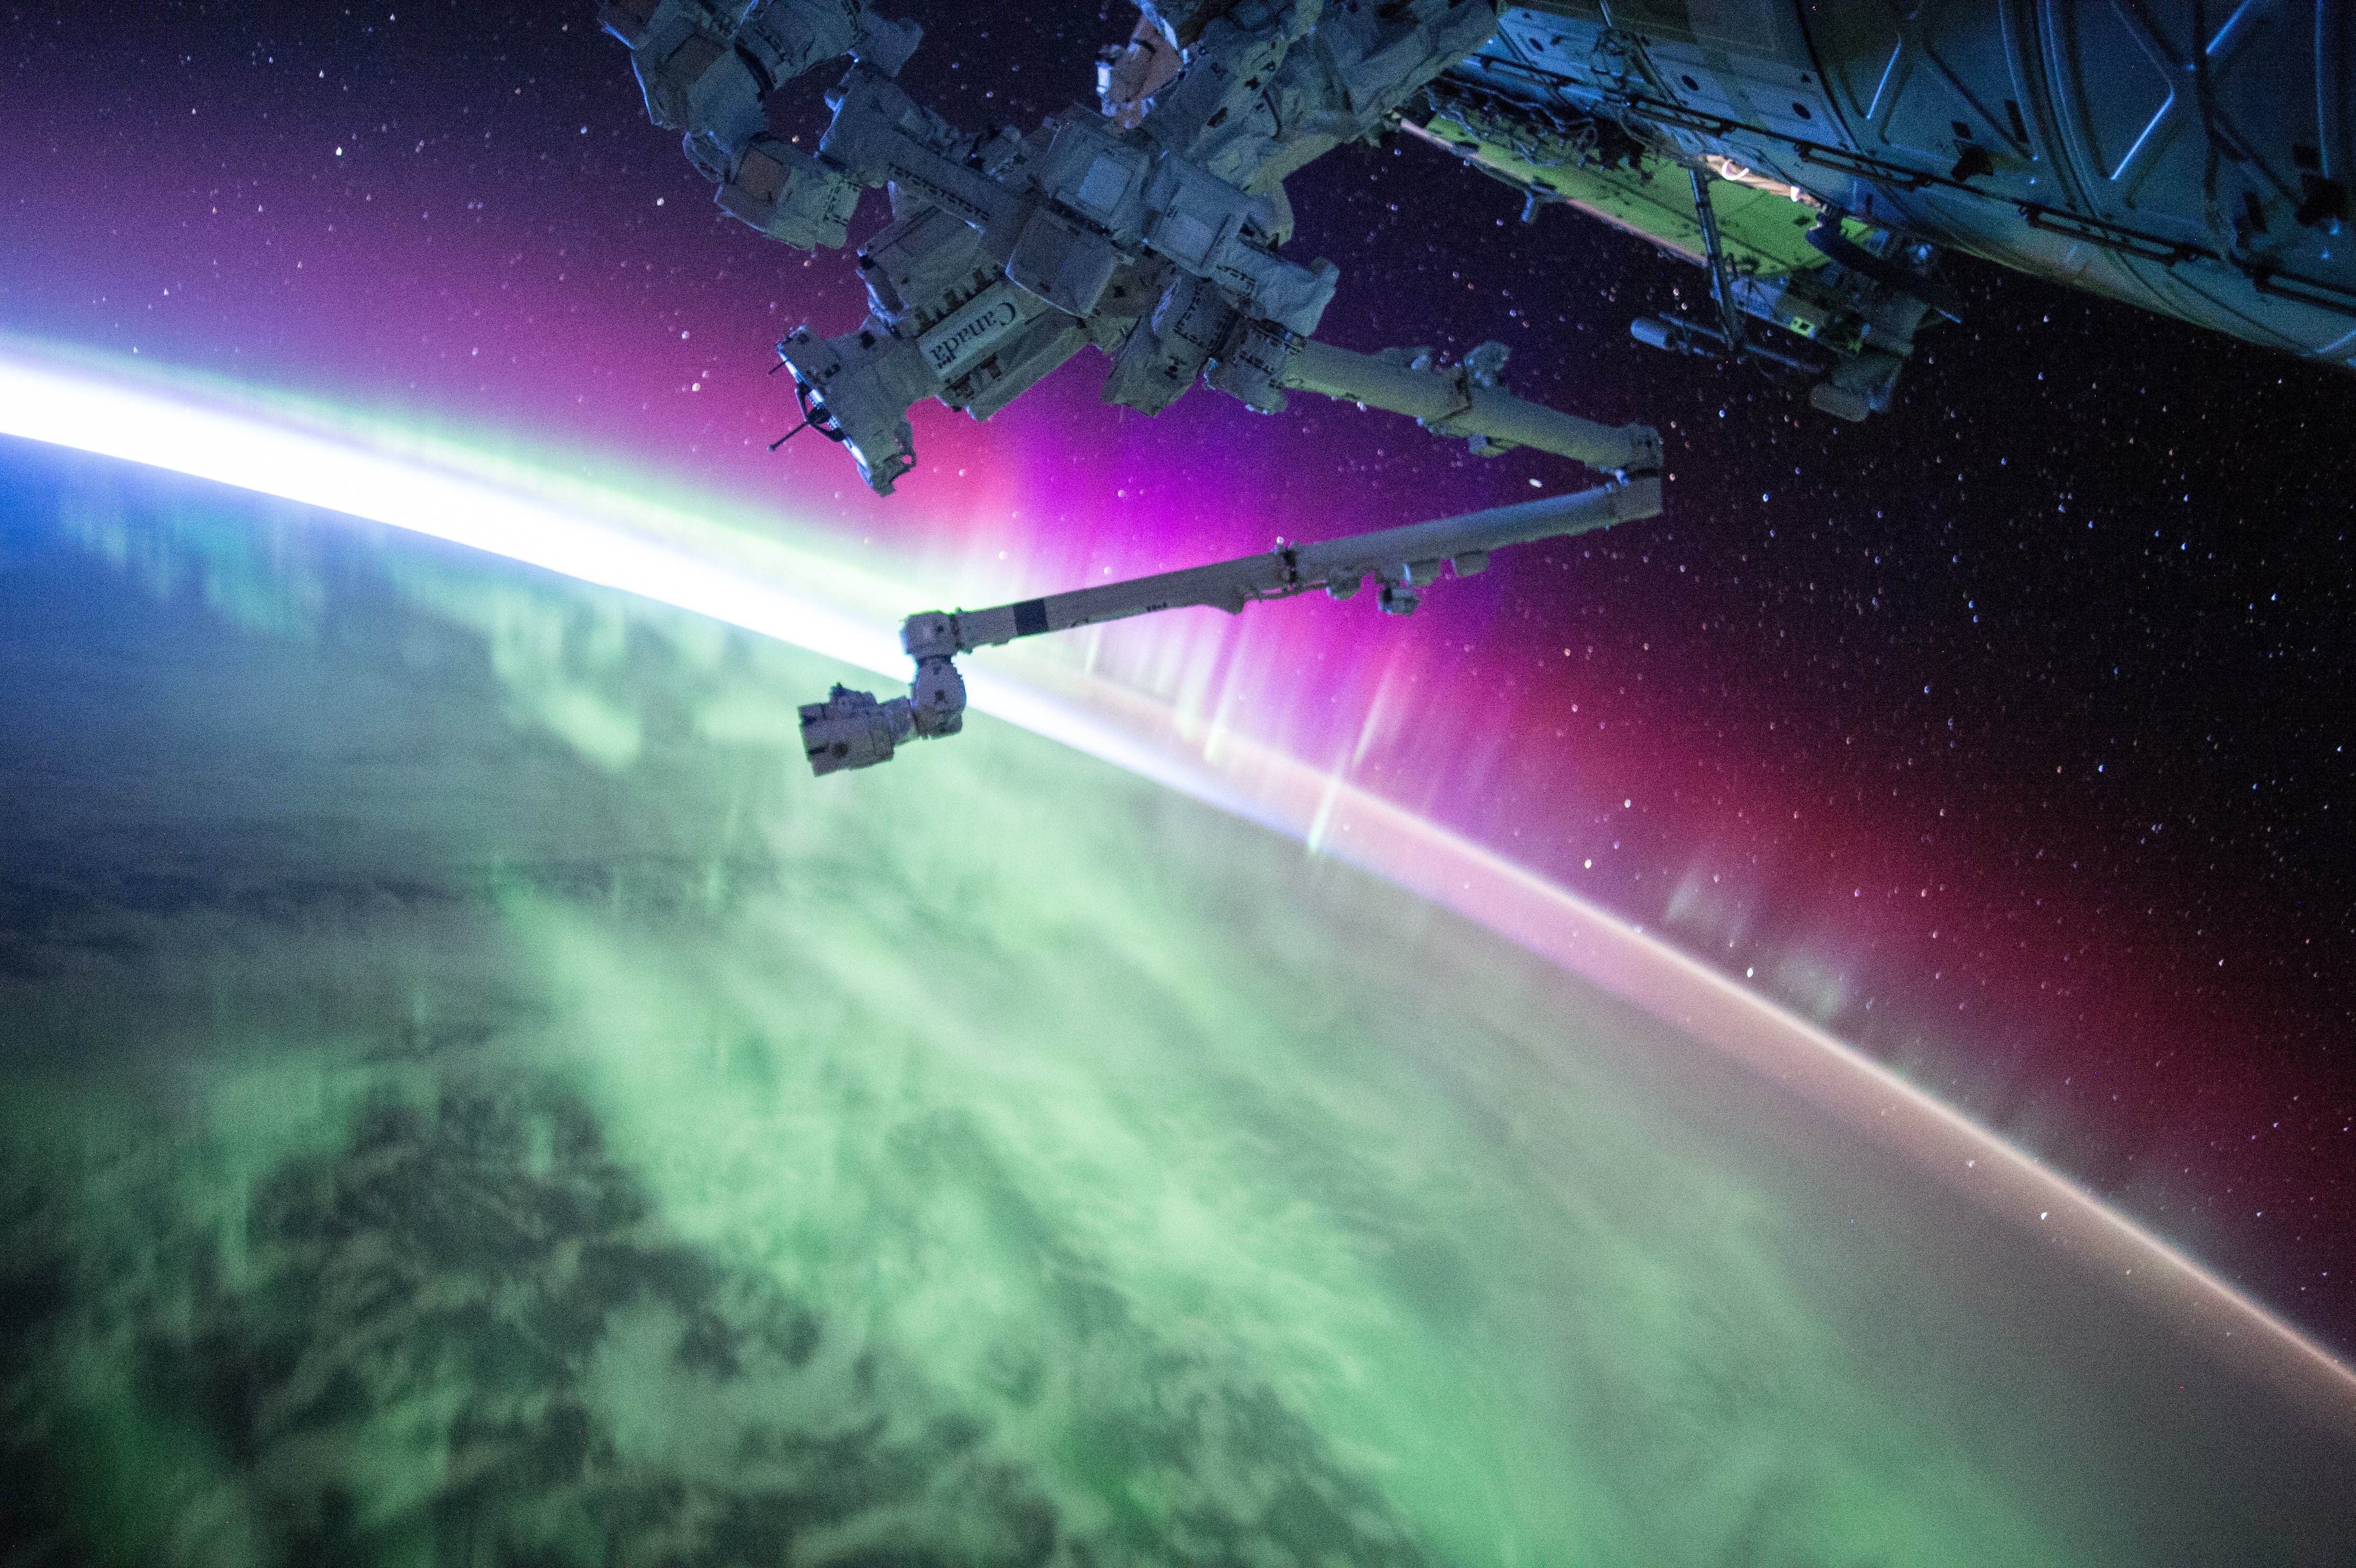
\includegraphics[scale=0.04]{Wellenausbreitung/Bilder/aurora.jpeg}
 \vspace{-6cm}
\end{wrapfigure}

\section*{Theorie- und Prüfungsfragen}

\begin{enumerate} 
\itemsep1pt\parskip0pt\parsep0pt
\item[1] Ergänze folgendes Schaubild: Abbildung  \ref{welle}. Tragen Sie die Bezeichnungen der einzelnen Schichten ein, die Höhe in der sie sich etwa befindet und die wichtigsten Frequenzen.
\end{enumerate}

\begin{figure}[H]
\def\svgwidth{\columnwidth}
\input{Wellenausbreitung/Bilder/Wellenausbreitung2.pdf_tex}
\caption{Aufbau der Ionosphäre und reflektierende Eigenschaften der Schichten}
\label{welle}
\end{figure}

% FIXME Hier muss markiert werden welche für die Prüfung wirklich wichtig sind!

\loesung{
\begin{figure}[H]
\def\svgwidth{\columnwidth}
\begin{wrapfigure}[0]{r}[-1cm]{4cm}
 \vspace{-6cm}
  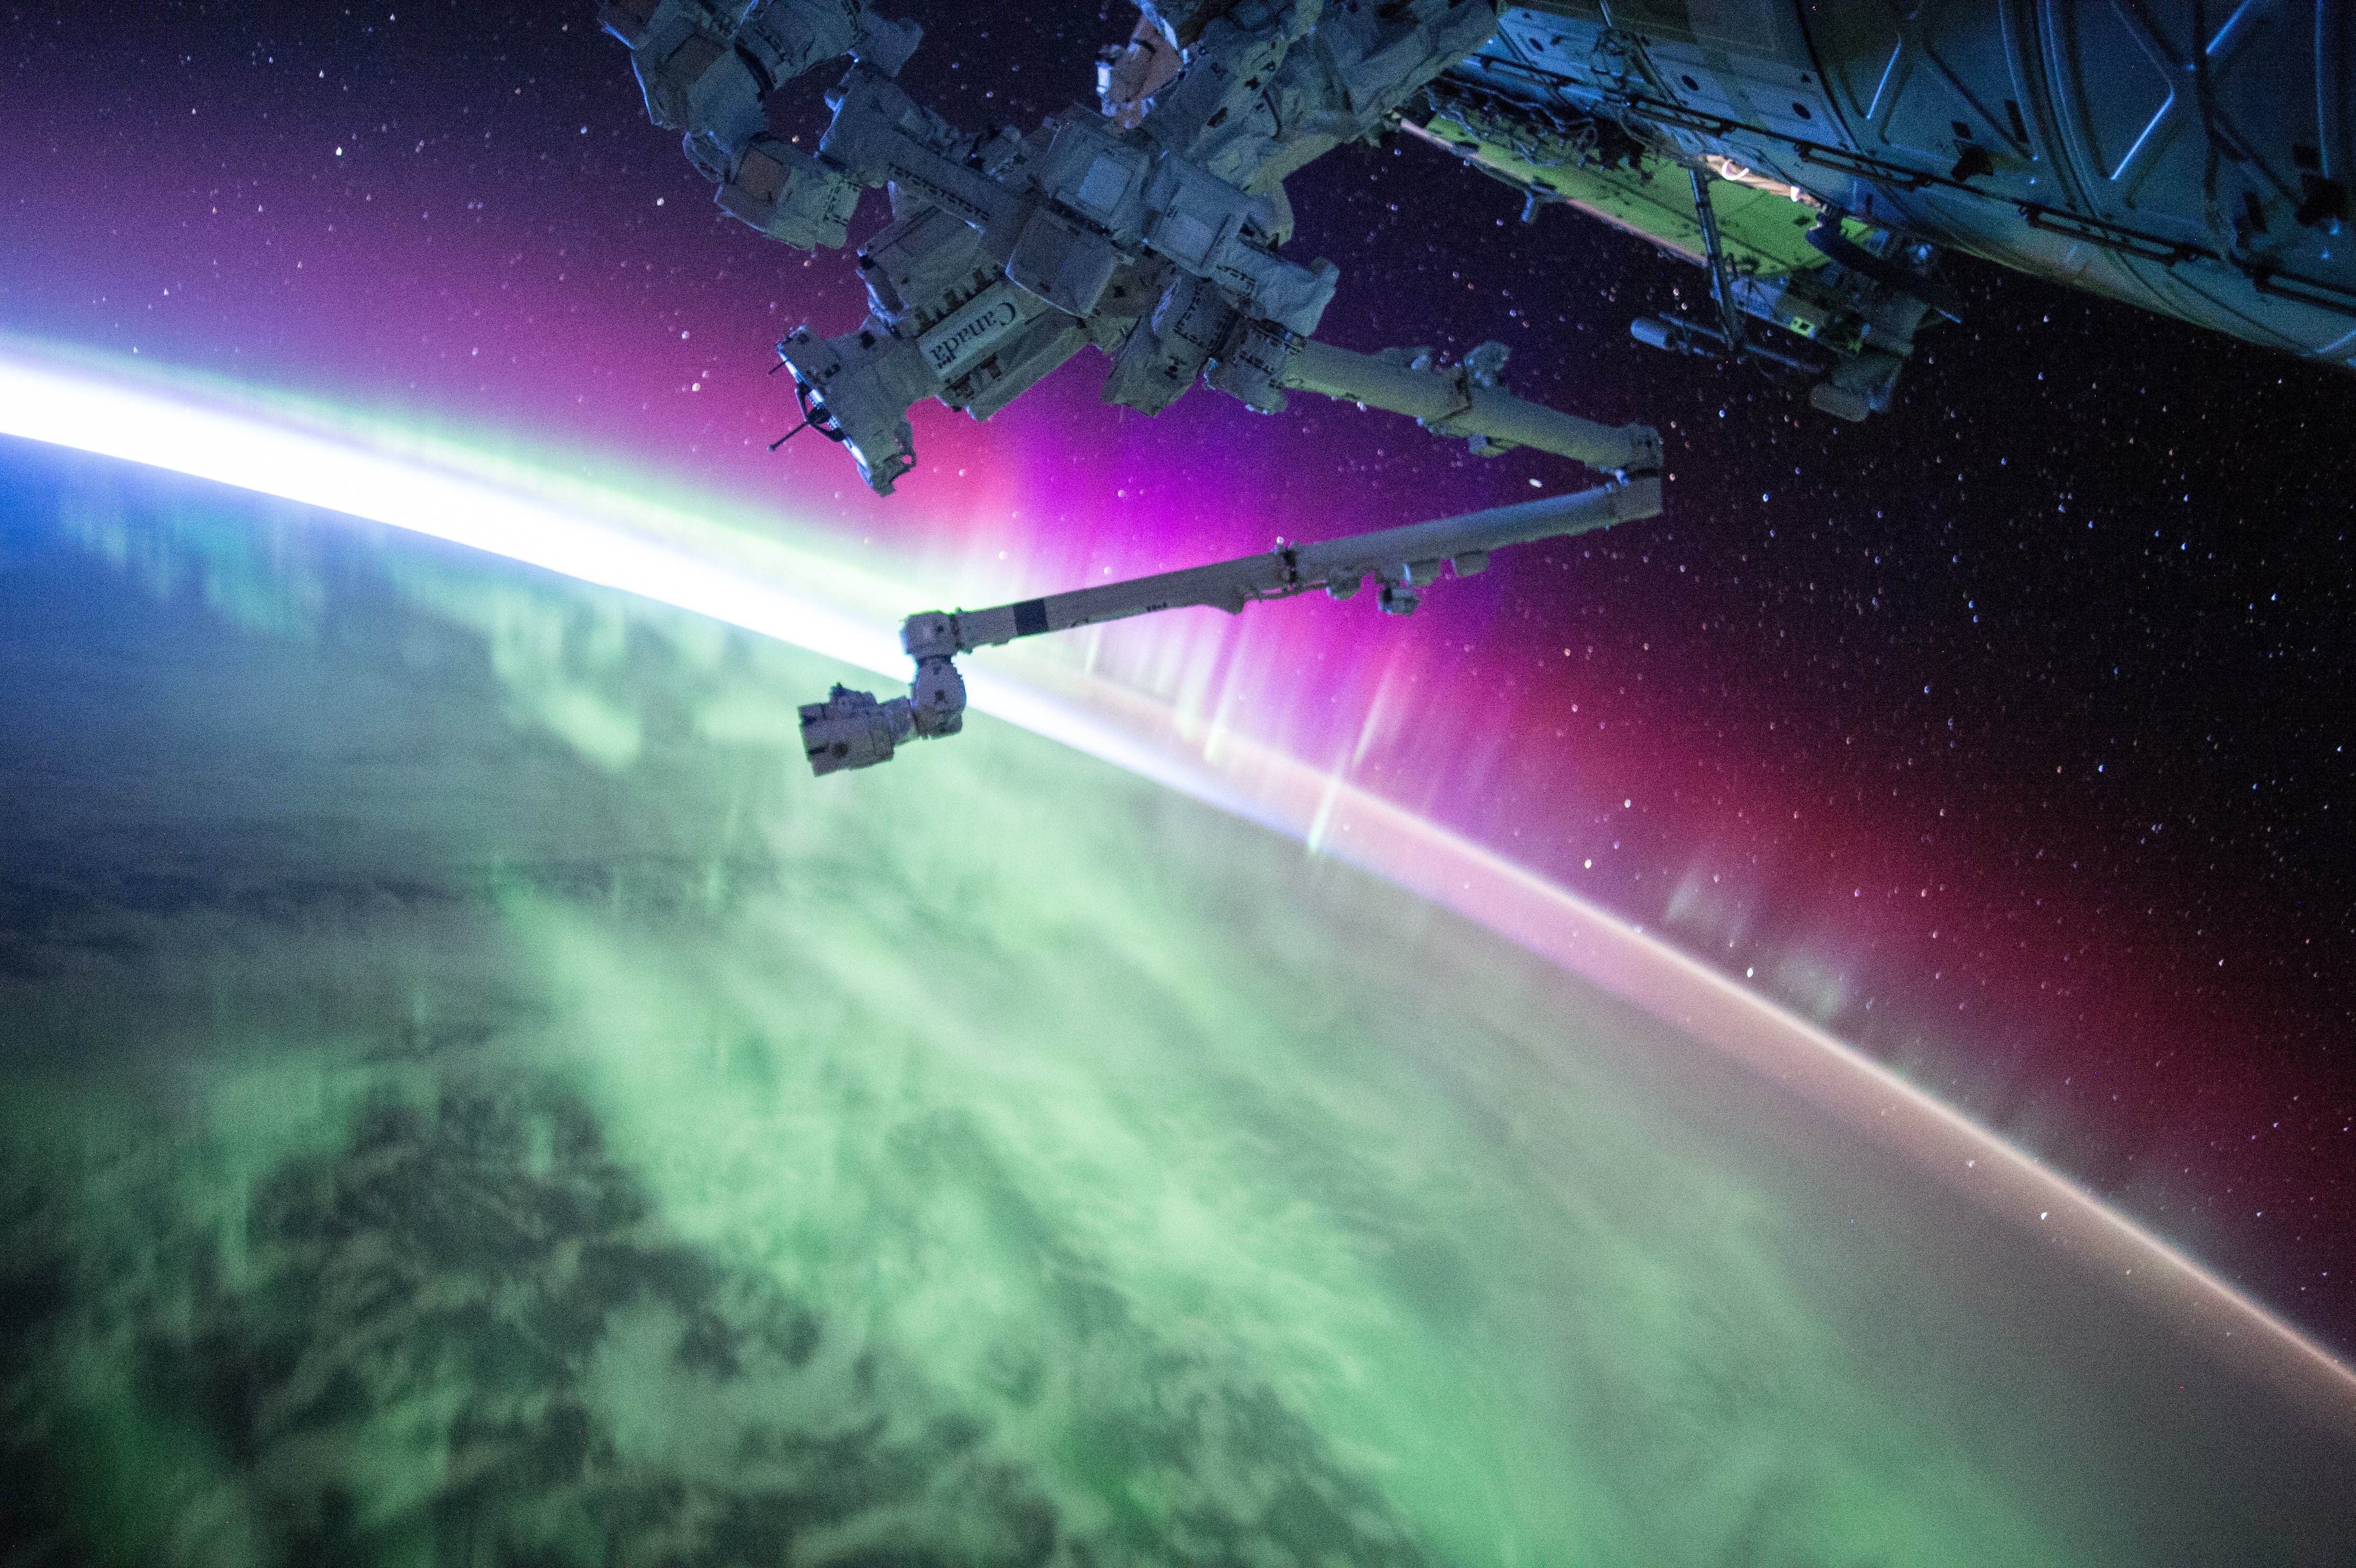
\includegraphics[scale=0.04]{Wellenausbreitung/Bilder/aurora.jpeg}
 \vspace{-6cm}
\end{wrapfigure}

\section*{Theorie- und Prüfungsfragen}

\begin{enumerate} 
\itemsep1pt\parskip0pt\parsep0pt
\item[1] Ergänze folgendes Schaubild: Abbildung  \ref{welle}. Tragen Sie die Bezeichnungen der einzelnen Schichten ein, die Höhe in der sie sich etwa befindet und die wichtigsten Frequenzen.
\end{enumerate}

\begin{figure}[H]
\def\svgwidth{\columnwidth}
\input{Wellenausbreitung/Bilder/Wellenausbreitung2.pdf_tex}
\caption{Aufbau der Ionosphäre und reflektierende Eigenschaften der Schichten}
\label{welle}
\end{figure}

% FIXME Hier muss markiert werden welche für die Prüfung wirklich wichtig sind!

\loesung{
\begin{figure}[H]
\def\svgwidth{\columnwidth}
\begin{wrapfigure}[0]{r}[-1cm]{4cm}
 \vspace{-6cm}
  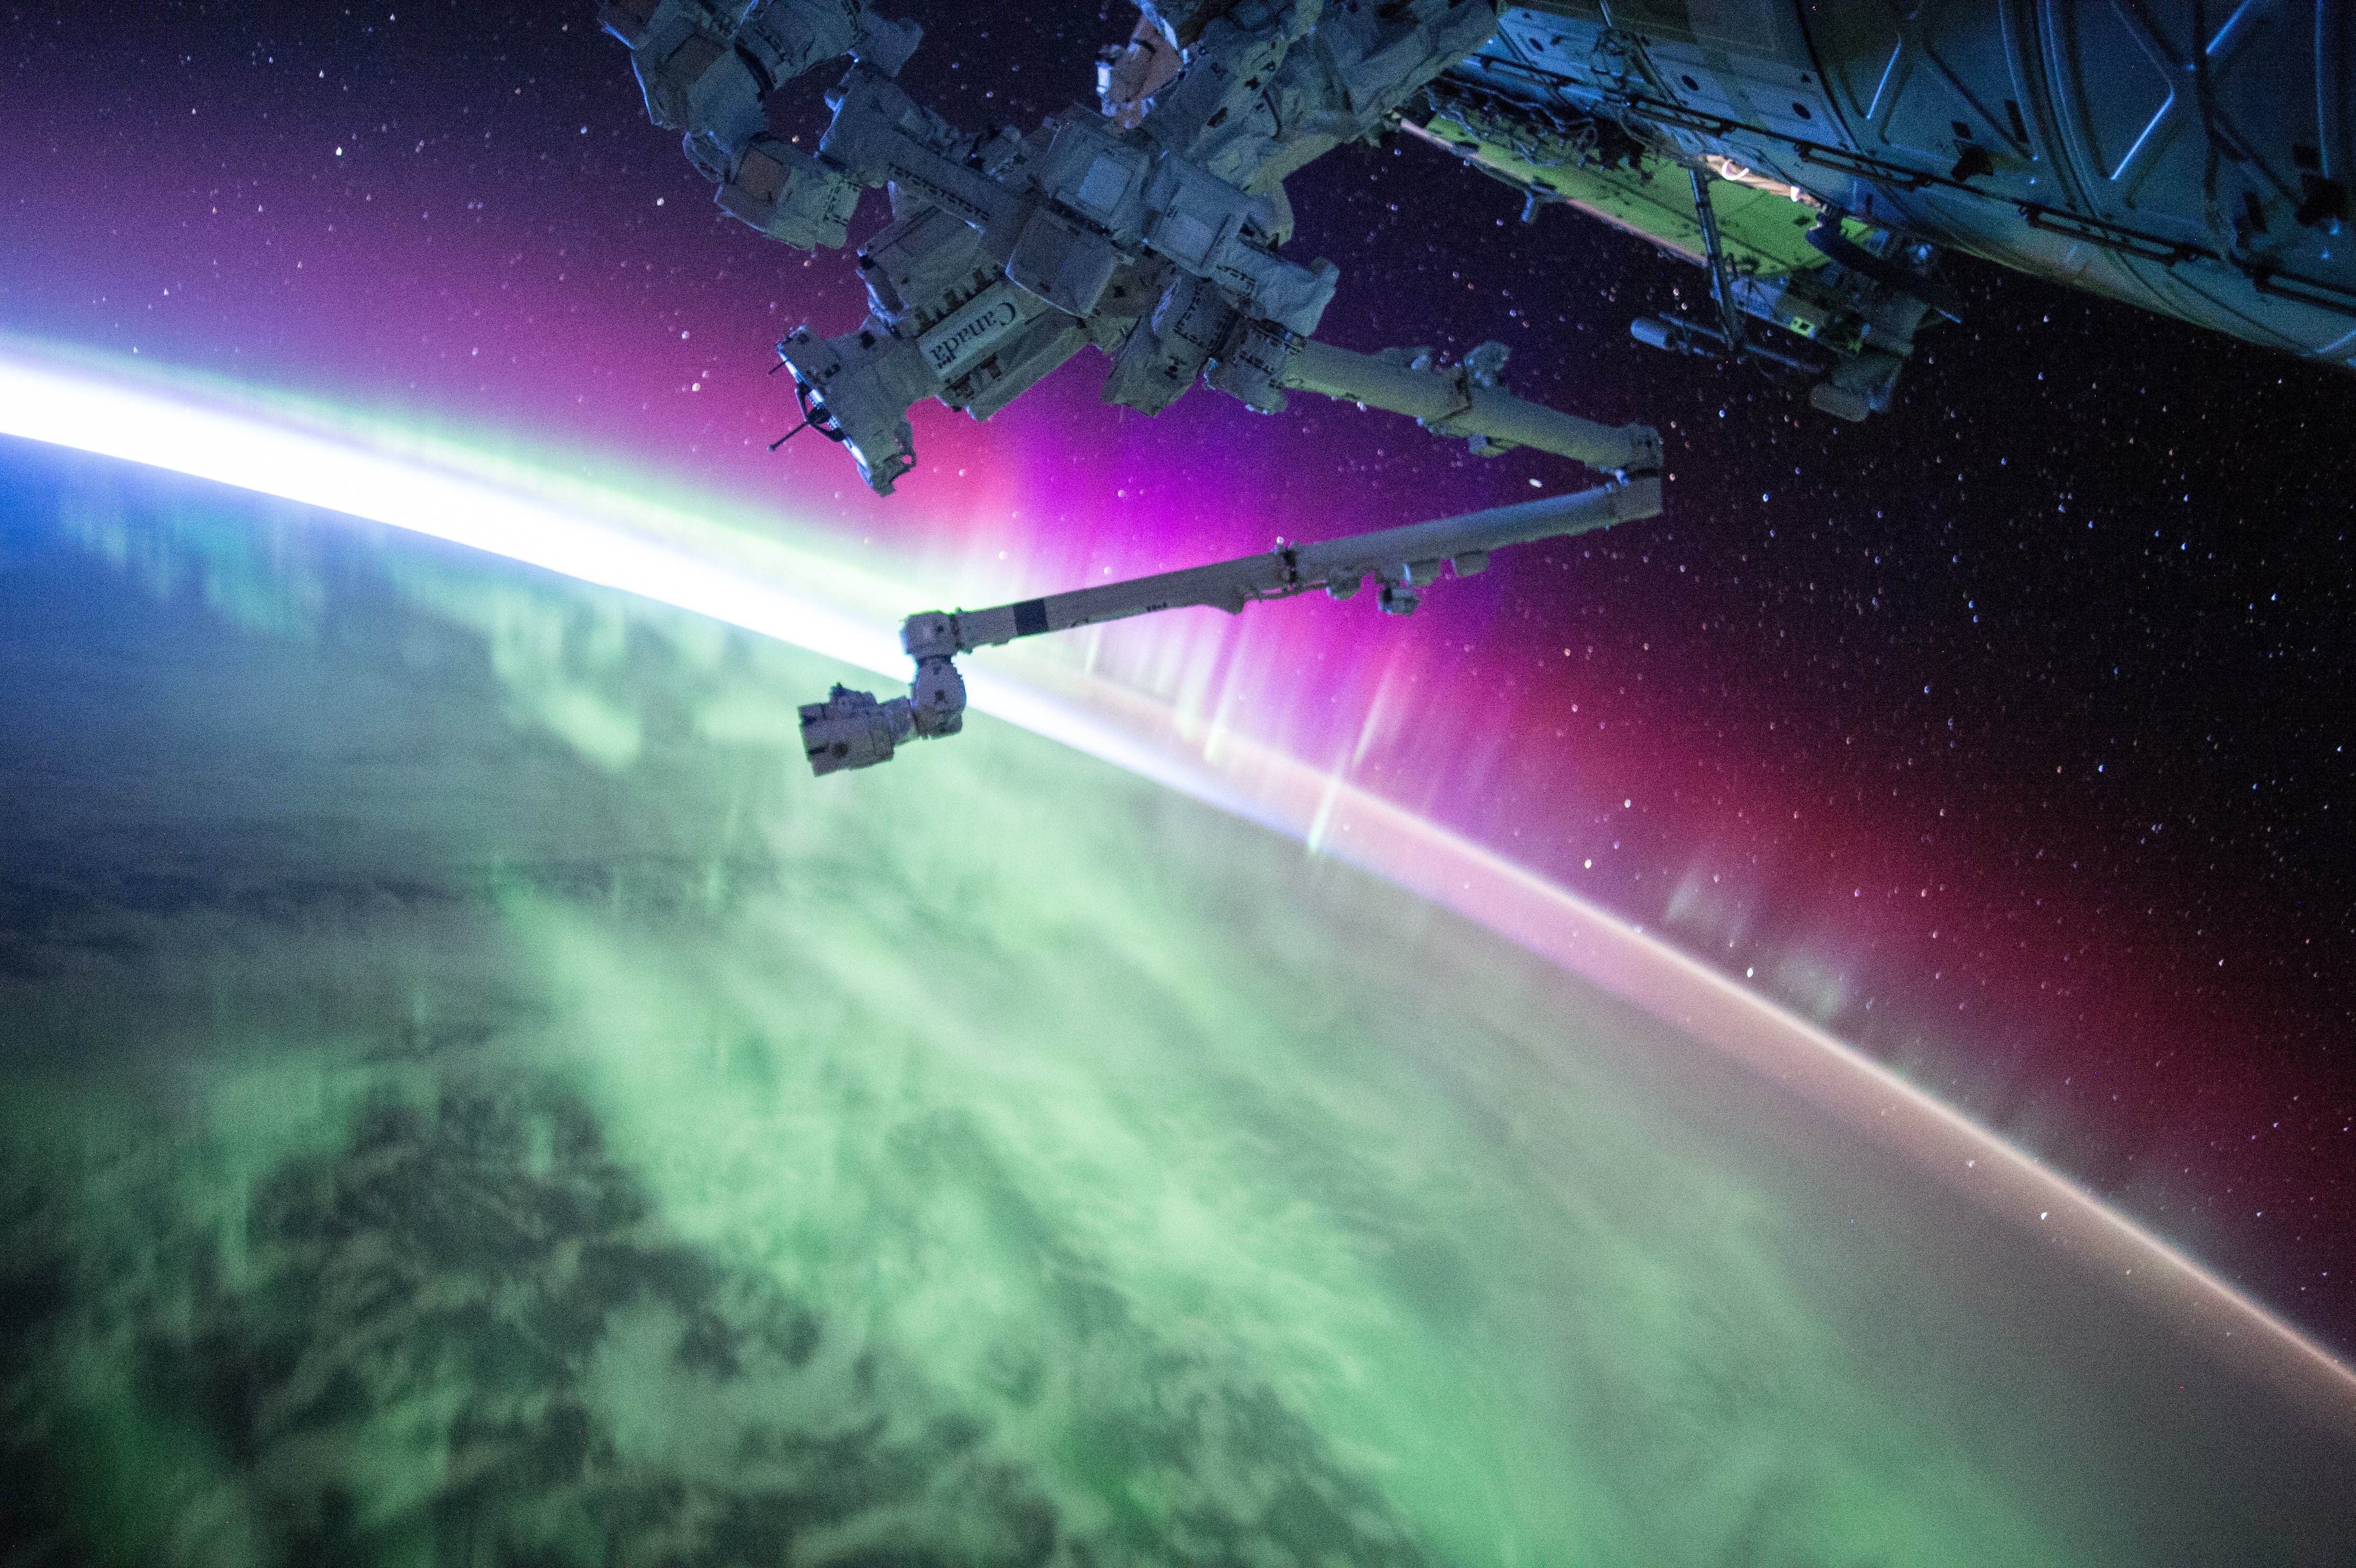
\includegraphics[scale=0.04]{Wellenausbreitung/Bilder/aurora.jpeg}
 \vspace{-6cm}
\end{wrapfigure}

\section*{Theorie- und Prüfungsfragen}

\begin{enumerate} 
\itemsep1pt\parskip0pt\parsep0pt
\item[1] Ergänze folgendes Schaubild: Abbildung  \ref{welle}. Tragen Sie die Bezeichnungen der einzelnen Schichten ein, die Höhe in der sie sich etwa befindet und die wichtigsten Frequenzen.
\end{enumerate}

\begin{figure}[H]
\def\svgwidth{\columnwidth}
\input{Wellenausbreitung/Bilder/Wellenausbreitung2.pdf_tex}
\caption{Aufbau der Ionosphäre und reflektierende Eigenschaften der Schichten}
\label{welle}
\end{figure}

% FIXME Hier muss markiert werden welche für die Prüfung wirklich wichtig sind!

\loesung{
\begin{figure}[H]
\def\svgwidth{\columnwidth}
\input{Wellenausbreitung/Bilder/Wellenausbreitung.pdf_tex}
\end{figure}
}

\begin{enumerate} 
\itemsep1pt\parskip0pt\parsep0pt
\item[2] \emph{\textbf{TI203}}  Welche der folgenden Aussagen trifft für KW-Funkverbindungen zu, die über Bodenwellen erfolgen? Die Bodenwelle folgt der Erdkrümmung und ...
	\begin{enumerate}
	\itemsep1pt\parskip0pt\parsep0pt
		\item[A] geht nicht über den geografischen Horizont hinaus. Sie wird in höheren Frequenzbereichen stärker gedämpft als in niedrigeren Frequenzbereichen.
		\item[B] geht über den geografischen Horizont hinaus. Sie wird in niedrigeren Frequenzbereichen stärker gedämpft als in höheren Frequenzbereichen.
		\item[C] geht über den geografischen Horizont hinaus. Sie wird in höheren Frequenzbereichen stärker gedämpft als in niedrigeren Frequenzbereichen.
		\item[D] geht nicht über den geografischen Horizont hinaus. Sie wird in niedrigeren Frequenzbereichen stärker gedämpft als in höheren Frequenzbereichen.
		\loesung{Lösung C}
	\end{enumerate}
\end{enumerate}

\begin{enumerate} 
\itemsep1pt\parskip0pt\parsep0pt
\item[3] \emph{\textbf{TI103}}  In welcher Höhe befinden sich die für die Fernausbreitung (DX) wichtigen ionosphärischen Schichten? Sie befinden sich in ungefähr ...
	\begin{enumerate}
	\itemsep1pt\parskip0pt\parsep0pt
		\item[A] 2 bis 5 km Höhe.
		\item[B] 20 bis 50 km Höhe.
		\item[C] 200 bis 500 km Höhe.
		\item[D] 2000 bis 5000 km Höhe.
		\loesung{Lösung C}
	\end{enumerate}
\end{enumerate}


\begin{enumerate} 
\itemsep1pt\parskip0pt\parsep0pt
\item[4] \emph{\textbf{TI107}}  Die Sonnenfleckenzahl ist einem regelmäßigen Zyklus unterworfen. Welchen Zeitraum hat dieser Zyklus zirka?
	\begin{enumerate}
	\itemsep1pt\parskip0pt\parsep0pt
		\item[A] 6 Monate
		\item[B] 12 Monate
		\item[C] 100 Jahre
		\item[D] 11 Jahre
	\loesung{Lösung D}
	\end{enumerate}
\end{enumerate}



\begin{enumerate} 
\itemsep1pt\parskip0pt\parsep0pt
\item[5] \emph{\textbf{TI212}}   Was bedeutet die $MUF$ bei der Kurzwellenausbreitung?
	\begin{enumerate}
	\itemsep1pt\parskip0pt\parsep0pt
		\item[A] Mittlere Nutzfrequenz
		\item[B] Höchste brauchbare Frequenz
		\item[C] Niedrigste brauchbare Frequenz
		\item[D] Kritische Grenzfrequenz
		\loesung{Lösung B}
	\end{enumerate}
\end{enumerate}

\begin{enumerate} 
\itemsep1pt\parskip0pt\parsep0pt
\item[6] \emph{\textbf{TI205}}   Von welchem der genannten Parameter ist die Sprungdistanz abhängig, die ein KW-Signal auf der Erdoberfläche überbrücken kann?
	\begin{enumerate}
	\itemsep1pt\parskip0pt\parsep0pt
		\item[A] Von der Polarisation der Antenne
		\item[B] Von der Sendeleistung
		\item[C] Vom Antennengewinn
		\item[D] Vom Abstrahlwinkel der Antenne
		\loesung{Lösung D}
	\end{enumerate}
\end{enumerate}


\begin{enumerate} 
\itemsep1pt\parskip0pt\parsep0pt
\item[7] \emph{\textbf{TI210}}   Warum sind Signale im 160- und 80-Meter-Band tagsüber nur schwach und nicht für den weltweiten Funkverkehr geeignet? Sie sind ungeeignet wegen der Tagesdämpfung in der ...
	\begin{enumerate}
	\itemsep1pt\parskip0pt\parsep0pt
		\item[A] A-Schicht
		\item[B] D-Schicht
		\item[C] F1-Schicht
		\item[D] F2-Schicht
		\loesung{Lösung B}
	\end{enumerate}
\end{enumerate}


\begin{enumerate} 
\itemsep1pt\parskip0pt\parsep0pt
\item[8] \emph{\textbf{TI106}}   Welche Schicht ist für die gute Ausbreitung im 10-m-Band in den Sommermonaten verantwortlich?
	\begin{enumerate}
	\itemsep1pt\parskip0pt\parsep0pt
		\item[A] D-Schicht
		\item[B] F1-Schicht
		\item[C] F2-Schicht
		\item[D] E-Schicht
		\loesung{Lösung D}
	\end{enumerate}
\end{enumerate}


\begin{enumerate} 
\itemsep1pt\parskip0pt\parsep0pt
\item[9] \emph{\textbf{TI202}}   Unter der ``Toten Zone'' wird der Bereich verstanden,
	\begin{enumerate}
	\itemsep1pt\parskip0pt\parsep0pt
		\item[A] der durch die Bodenwelle überdeckt wird, so dass schwächere DX-Stationen zugedeckt werden.
		\item[B] der durch die Bodenwelle erreicht wird und für die Raumwelle nicht zugänglich ist.
		\item[C] der durch die Bodenwelle nicht mehr erreicht wird und durch die reflektierte Raumwelle noch nicht erreicht wird.
		\item[D] der durch die Interferenz der Bodenwelle mit der Raumwelle in einer Zone der gegenseitigen Auslöschung liegt.
		\loesung{Lösung C}
	\end{enumerate}
\end{enumerate}

\begin{enumerate} 
\itemsep1pt\parskip0pt\parsep0pt
\item[10] \emph{\textbf{TI206}}   Bei der Ausbreitung auf Kurzwelle spielt die so genannte ``Grey Line'' eine besondere Rolle. Was ist die ``Grey Line''?
	\begin{enumerate}
	\itemsep1pt\parskip0pt\parsep0pt
		\item[A] Die instabilen Ausbreitungsbedingungen in der Äquatorialzone.
		\item[B] Die Zeit mit den besten Möglichkeiten für ``Short Skip'' Ausbreitung.
		\item[C] Die Übergangszeit vor und nach dem Winter, in der sich die D-Schicht ab- und wieder aufbaut.
		\item[D] Der Streifen der Dämmerungsphase vor Sonnenaufgang oder nach Sonnenuntergang.
		\loesung{Lösung D}
	\end{enumerate}
\end{enumerate}

\begin{enumerate} 
\itemsep1pt\parskip0pt\parsep0pt
\item[11] Ergänze in der Tabelle die jeweiligen Frequenzbereiche für die einzelnen Bänder.
\end{enumerate}


\begin{figure}[H]
	\subfigure{
		\begin{tabular}{|r|l|}
			\hline
			Band 	& Frequenzbereich\\
			\hline
			$160m$ & ~\hspace*{4cm}\\
			$80m$  & ~\hspace*{4cm}\\
			$40m$  & ~\hspace*{4cm}\\
			$20m$  & ~\hspace*{4cm}\\
			$15m$  & ~\hspace*{4cm}\\
			$10m$  & ~\hspace*{4cm}\\
			\hline
		\end{tabular}
	}
	\subfigure{
		\loesung{
			\begin{tabular}{|r|l|}
				\hline
				Band 	& Frequenzbereich\\
				\hline
				$160m$ & $1,810-2,000MHz$\\
				$80m$  & $3,500-3,800MHz$\\
				$40m$  & $7,000-7,200MHz$\\
				$20m$  & $14,000-14,350MHz$\\
				$15m$  & $21,000-21,450MHz$\\
				$10m$  & $28,000-29,700MHz$\\
				\hline
			\end{tabular}
			}
	}
\end{figure}


\begin{enumerate} 
\itemsep1pt\parskip0pt\parsep0pt
\item[12] \emph{\textbf{TI210}}   Warum sind Signale im 160- und 80-Meter-Band tagsüber nur schwach und nicht für den weltweiten Funkverkehr geeignet? Sie sind ungeeignet wegen der Tagesdämpfung in der
	\begin{enumerate}
	\itemsep1pt\parskip0pt\parsep0pt
		\item[A] A-Schicht
		\item[B] D-Schicht
		\item[C] F1-Schicht
		\item[D] F2-Schicht
		\loesung{Lösung B}
	\end{enumerate}
\end{enumerate}


\begin{enumerate} 
\itemsep1pt\parskip0pt\parsep0pt
\item[13] \emph{\textbf{TI301}}   Wie weit etwa reicht der Funkhorizont im UKW-Bereich über den geografischen Horizont hinaus? Er reicht etwa ...
	\begin{enumerate}
	\itemsep1pt\parskip0pt\parsep0pt
		\item[A] doppelt so weit.
		\item[B] bis zur Hälfte der Entfernung bis zum geografischen Horizont.
		\item[C] bis zum Vierfachen der Entfernung bis zum geografischen Horizont.
		\item[D] $15 \%$ weiter als der geografische Horizont.
		\loesung{Lösung D}
	\end{enumerate}
\end{enumerate}

\begin{enumerate} 
\itemsep1pt\parskip0pt\parsep0pt
\item[14] \emph{\textbf{TI305}}   Wie wirkt die Antennenhöhe auf die Reichweite einer UKW-Verbindung aus? Die Reichweite steigt mit zunehmender Antennenhöhe, weil ...
	\begin{enumerate}
	\itemsep1pt\parskip0pt\parsep0pt
		\item[A] die dämpfende Wirkung der Erdoberfläche abnimmt.
		\item[B] die Entfernung zu den reflektierenden Schichten der Troposphäre abnimmt.
		\item[C] in höheren Luftschichten die Temperatur sinkt.
		\item[D] die optische Sichtweite zunimmt.
		\loesung{Lösung D}
	\end{enumerate}
\end{enumerate}


\begin{enumerate} 
\itemsep1pt\parskip0pt\parsep0pt
\item[15] \emph{\textbf{TI309}}   Was versteht man unter dem Begriff Sporadic E? Man versteht darunter ...
	\begin{enumerate}
	\itemsep1pt\parskip0pt\parsep0pt
		\item[A] kurzfristige plötzliche Inversionsänderungen in der E-Schicht, die Fernausbreitung im VHF-Bereich ermöglichen.
		\item[B] kurzzeitig auftretende starke Reflexion von VHF-Signalen an Meteorbahnen innerhalb der E-Schicht.
		\item[C] lokal begrenzten kurzzeitigen Ausfall der Reflexion durch ungewöhnlich hohe Ionisation innerhalb der E-Schicht.
		\item[D] die Reflexion an lokal begrenzten Bereichen mit ungewöhnlich hoher Ionisation innerhalb der E-Schicht.
		\loesung{Lösung D}
	\end{enumerate}
\end{enumerate}

\begin{enumerate} 
\itemsep1pt\parskip0pt\parsep0pt
\item[16] \emph{\textbf{TI204}}  Wie groß ist in etwa die maximale Entfernung, die ein KW-Signal bei Reflexion an der E-Schicht auf der Erdoberfläche mit einem Sprung (Hop) überbrücken kann?
	\begin{enumerate}
	\itemsep1pt\parskip0pt\parsep0pt
		\item[A] Etwa 1100 km
		\item[B] Etwa 2200 km
		\item[C] Etwa 4500 km
		\item[D] Etwa 9000 km
		\loesung{Lösung B}
	\end{enumerate}
\end{enumerate}


\begin{enumerate} 
\itemsep1pt\parskip0pt\parsep0pt
\item[17] \emph{\textbf{TI211}}   In welcher ionosphärischen Schicht treten gelegentlich Aurora-Erscheinungen auf?
	\begin{enumerate}
	\itemsep1pt\parskip0pt\parsep0pt
		\item[A] In der F-Schicht
		\item[B] In der E-Schicht Nähe des Äquators
		\item[C] In der E-Schicht
		\item[D] In der D-Schicht
		\loesung{Lösung C}
	\end{enumerate}
\end{enumerate}

\begin{enumerate} 
\itemsep1pt\parskip0pt\parsep0pt
\item[18] \emph{\textbf{TI306}} Was ist die Ursache für Aurora-Erscheinungen? Die Ursache ist ...
	\begin{enumerate}
	\itemsep1pt\parskip0pt\parsep0pt
		\item[A] das Eindringen geladener Teilchen von der Sonne in die Atmosphäre.
		\item[B] eine hohe Sonnenfleckenzahl.
		\item[C] eine niedrige Sonnenfleckenzahl.
		\item[D] das Auftreten von Meteoritenschauern in den polaren Regionen.
		\loesung{Lösung A}
	\end{enumerate}
\end{enumerate}

\begin{enumerate} 
\itemsep1pt\parskip0pt\parsep0pt
\item[19] \emph{\textbf{TI307}} Wie wirkt sich Aurora auf die Signalqualität eines Funksignals aus?
	\begin{enumerate}
	\itemsep1pt\parskip0pt\parsep0pt
		\item[A] CW-Signale haben einen flatternden und verbrummten Ton.
		\item[B] CW- Signale haben einen besseren Ton.
		\item[C] Die Lesbarkeit der SSB-Signale verbessert sich.
		\item[D] Die Lesbarkeit der FM-Signale verbessert sich.
		\loesung{Lösung A}
	\end{enumerate}
\end{enumerate}

\end{figure}
}

\begin{enumerate} 
\itemsep1pt\parskip0pt\parsep0pt
\item[2] \emph{\textbf{TI203}}  Welche der folgenden Aussagen trifft für KW-Funkverbindungen zu, die über Bodenwellen erfolgen? Die Bodenwelle folgt der Erdkrümmung und ...
	\begin{enumerate}
	\itemsep1pt\parskip0pt\parsep0pt
		\item[A] geht nicht über den geografischen Horizont hinaus. Sie wird in höheren Frequenzbereichen stärker gedämpft als in niedrigeren Frequenzbereichen.
		\item[B] geht über den geografischen Horizont hinaus. Sie wird in niedrigeren Frequenzbereichen stärker gedämpft als in höheren Frequenzbereichen.
		\item[C] geht über den geografischen Horizont hinaus. Sie wird in höheren Frequenzbereichen stärker gedämpft als in niedrigeren Frequenzbereichen.
		\item[D] geht nicht über den geografischen Horizont hinaus. Sie wird in niedrigeren Frequenzbereichen stärker gedämpft als in höheren Frequenzbereichen.
		\loesung{Lösung C}
	\end{enumerate}
\end{enumerate}

\begin{enumerate} 
\itemsep1pt\parskip0pt\parsep0pt
\item[3] \emph{\textbf{TI103}}  In welcher Höhe befinden sich die für die Fernausbreitung (DX) wichtigen ionosphärischen Schichten? Sie befinden sich in ungefähr ...
	\begin{enumerate}
	\itemsep1pt\parskip0pt\parsep0pt
		\item[A] 2 bis 5 km Höhe.
		\item[B] 20 bis 50 km Höhe.
		\item[C] 200 bis 500 km Höhe.
		\item[D] 2000 bis 5000 km Höhe.
		\loesung{Lösung C}
	\end{enumerate}
\end{enumerate}


\begin{enumerate} 
\itemsep1pt\parskip0pt\parsep0pt
\item[4] \emph{\textbf{TI107}}  Die Sonnenfleckenzahl ist einem regelmäßigen Zyklus unterworfen. Welchen Zeitraum hat dieser Zyklus zirka?
	\begin{enumerate}
	\itemsep1pt\parskip0pt\parsep0pt
		\item[A] 6 Monate
		\item[B] 12 Monate
		\item[C] 100 Jahre
		\item[D] 11 Jahre
	\loesung{Lösung D}
	\end{enumerate}
\end{enumerate}



\begin{enumerate} 
\itemsep1pt\parskip0pt\parsep0pt
\item[5] \emph{\textbf{TI212}}   Was bedeutet die $MUF$ bei der Kurzwellenausbreitung?
	\begin{enumerate}
	\itemsep1pt\parskip0pt\parsep0pt
		\item[A] Mittlere Nutzfrequenz
		\item[B] Höchste brauchbare Frequenz
		\item[C] Niedrigste brauchbare Frequenz
		\item[D] Kritische Grenzfrequenz
		\loesung{Lösung B}
	\end{enumerate}
\end{enumerate}

\begin{enumerate} 
\itemsep1pt\parskip0pt\parsep0pt
\item[6] \emph{\textbf{TI205}}   Von welchem der genannten Parameter ist die Sprungdistanz abhängig, die ein KW-Signal auf der Erdoberfläche überbrücken kann?
	\begin{enumerate}
	\itemsep1pt\parskip0pt\parsep0pt
		\item[A] Von der Polarisation der Antenne
		\item[B] Von der Sendeleistung
		\item[C] Vom Antennengewinn
		\item[D] Vom Abstrahlwinkel der Antenne
		\loesung{Lösung D}
	\end{enumerate}
\end{enumerate}


\begin{enumerate} 
\itemsep1pt\parskip0pt\parsep0pt
\item[7] \emph{\textbf{TI210}}   Warum sind Signale im 160- und 80-Meter-Band tagsüber nur schwach und nicht für den weltweiten Funkverkehr geeignet? Sie sind ungeeignet wegen der Tagesdämpfung in der ...
	\begin{enumerate}
	\itemsep1pt\parskip0pt\parsep0pt
		\item[A] A-Schicht
		\item[B] D-Schicht
		\item[C] F1-Schicht
		\item[D] F2-Schicht
		\loesung{Lösung B}
	\end{enumerate}
\end{enumerate}


\begin{enumerate} 
\itemsep1pt\parskip0pt\parsep0pt
\item[8] \emph{\textbf{TI106}}   Welche Schicht ist für die gute Ausbreitung im 10-m-Band in den Sommermonaten verantwortlich?
	\begin{enumerate}
	\itemsep1pt\parskip0pt\parsep0pt
		\item[A] D-Schicht
		\item[B] F1-Schicht
		\item[C] F2-Schicht
		\item[D] E-Schicht
		\loesung{Lösung D}
	\end{enumerate}
\end{enumerate}


\begin{enumerate} 
\itemsep1pt\parskip0pt\parsep0pt
\item[9] \emph{\textbf{TI202}}   Unter der ``Toten Zone'' wird der Bereich verstanden,
	\begin{enumerate}
	\itemsep1pt\parskip0pt\parsep0pt
		\item[A] der durch die Bodenwelle überdeckt wird, so dass schwächere DX-Stationen zugedeckt werden.
		\item[B] der durch die Bodenwelle erreicht wird und für die Raumwelle nicht zugänglich ist.
		\item[C] der durch die Bodenwelle nicht mehr erreicht wird und durch die reflektierte Raumwelle noch nicht erreicht wird.
		\item[D] der durch die Interferenz der Bodenwelle mit der Raumwelle in einer Zone der gegenseitigen Auslöschung liegt.
		\loesung{Lösung C}
	\end{enumerate}
\end{enumerate}

\begin{enumerate} 
\itemsep1pt\parskip0pt\parsep0pt
\item[10] \emph{\textbf{TI206}}   Bei der Ausbreitung auf Kurzwelle spielt die so genannte ``Grey Line'' eine besondere Rolle. Was ist die ``Grey Line''?
	\begin{enumerate}
	\itemsep1pt\parskip0pt\parsep0pt
		\item[A] Die instabilen Ausbreitungsbedingungen in der Äquatorialzone.
		\item[B] Die Zeit mit den besten Möglichkeiten für ``Short Skip'' Ausbreitung.
		\item[C] Die Übergangszeit vor und nach dem Winter, in der sich die D-Schicht ab- und wieder aufbaut.
		\item[D] Der Streifen der Dämmerungsphase vor Sonnenaufgang oder nach Sonnenuntergang.
		\loesung{Lösung D}
	\end{enumerate}
\end{enumerate}

\begin{enumerate} 
\itemsep1pt\parskip0pt\parsep0pt
\item[11] Ergänze in der Tabelle die jeweiligen Frequenzbereiche für die einzelnen Bänder.
\end{enumerate}


\begin{figure}[H]
	\subfigure{
		\begin{tabular}{|r|l|}
			\hline
			Band 	& Frequenzbereich\\
			\hline
			$160m$ & ~\hspace*{4cm}\\
			$80m$  & ~\hspace*{4cm}\\
			$40m$  & ~\hspace*{4cm}\\
			$20m$  & ~\hspace*{4cm}\\
			$15m$  & ~\hspace*{4cm}\\
			$10m$  & ~\hspace*{4cm}\\
			\hline
		\end{tabular}
	}
	\subfigure{
		\loesung{
			\begin{tabular}{|r|l|}
				\hline
				Band 	& Frequenzbereich\\
				\hline
				$160m$ & $1,810-2,000MHz$\\
				$80m$  & $3,500-3,800MHz$\\
				$40m$  & $7,000-7,200MHz$\\
				$20m$  & $14,000-14,350MHz$\\
				$15m$  & $21,000-21,450MHz$\\
				$10m$  & $28,000-29,700MHz$\\
				\hline
			\end{tabular}
			}
	}
\end{figure}


\begin{enumerate} 
\itemsep1pt\parskip0pt\parsep0pt
\item[12] \emph{\textbf{TI210}}   Warum sind Signale im 160- und 80-Meter-Band tagsüber nur schwach und nicht für den weltweiten Funkverkehr geeignet? Sie sind ungeeignet wegen der Tagesdämpfung in der
	\begin{enumerate}
	\itemsep1pt\parskip0pt\parsep0pt
		\item[A] A-Schicht
		\item[B] D-Schicht
		\item[C] F1-Schicht
		\item[D] F2-Schicht
		\loesung{Lösung B}
	\end{enumerate}
\end{enumerate}


\begin{enumerate} 
\itemsep1pt\parskip0pt\parsep0pt
\item[13] \emph{\textbf{TI301}}   Wie weit etwa reicht der Funkhorizont im UKW-Bereich über den geografischen Horizont hinaus? Er reicht etwa ...
	\begin{enumerate}
	\itemsep1pt\parskip0pt\parsep0pt
		\item[A] doppelt so weit.
		\item[B] bis zur Hälfte der Entfernung bis zum geografischen Horizont.
		\item[C] bis zum Vierfachen der Entfernung bis zum geografischen Horizont.
		\item[D] $15 \%$ weiter als der geografische Horizont.
		\loesung{Lösung D}
	\end{enumerate}
\end{enumerate}

\begin{enumerate} 
\itemsep1pt\parskip0pt\parsep0pt
\item[14] \emph{\textbf{TI305}}   Wie wirkt die Antennenhöhe auf die Reichweite einer UKW-Verbindung aus? Die Reichweite steigt mit zunehmender Antennenhöhe, weil ...
	\begin{enumerate}
	\itemsep1pt\parskip0pt\parsep0pt
		\item[A] die dämpfende Wirkung der Erdoberfläche abnimmt.
		\item[B] die Entfernung zu den reflektierenden Schichten der Troposphäre abnimmt.
		\item[C] in höheren Luftschichten die Temperatur sinkt.
		\item[D] die optische Sichtweite zunimmt.
		\loesung{Lösung D}
	\end{enumerate}
\end{enumerate}


\begin{enumerate} 
\itemsep1pt\parskip0pt\parsep0pt
\item[15] \emph{\textbf{TI309}}   Was versteht man unter dem Begriff Sporadic E? Man versteht darunter ...
	\begin{enumerate}
	\itemsep1pt\parskip0pt\parsep0pt
		\item[A] kurzfristige plötzliche Inversionsänderungen in der E-Schicht, die Fernausbreitung im VHF-Bereich ermöglichen.
		\item[B] kurzzeitig auftretende starke Reflexion von VHF-Signalen an Meteorbahnen innerhalb der E-Schicht.
		\item[C] lokal begrenzten kurzzeitigen Ausfall der Reflexion durch ungewöhnlich hohe Ionisation innerhalb der E-Schicht.
		\item[D] die Reflexion an lokal begrenzten Bereichen mit ungewöhnlich hoher Ionisation innerhalb der E-Schicht.
		\loesung{Lösung D}
	\end{enumerate}
\end{enumerate}

\begin{enumerate} 
\itemsep1pt\parskip0pt\parsep0pt
\item[16] \emph{\textbf{TI204}}  Wie groß ist in etwa die maximale Entfernung, die ein KW-Signal bei Reflexion an der E-Schicht auf der Erdoberfläche mit einem Sprung (Hop) überbrücken kann?
	\begin{enumerate}
	\itemsep1pt\parskip0pt\parsep0pt
		\item[A] Etwa 1100 km
		\item[B] Etwa 2200 km
		\item[C] Etwa 4500 km
		\item[D] Etwa 9000 km
		\loesung{Lösung B}
	\end{enumerate}
\end{enumerate}


\begin{enumerate} 
\itemsep1pt\parskip0pt\parsep0pt
\item[17] \emph{\textbf{TI211}}   In welcher ionosphärischen Schicht treten gelegentlich Aurora-Erscheinungen auf?
	\begin{enumerate}
	\itemsep1pt\parskip0pt\parsep0pt
		\item[A] In der F-Schicht
		\item[B] In der E-Schicht Nähe des Äquators
		\item[C] In der E-Schicht
		\item[D] In der D-Schicht
		\loesung{Lösung C}
	\end{enumerate}
\end{enumerate}

\begin{enumerate} 
\itemsep1pt\parskip0pt\parsep0pt
\item[18] \emph{\textbf{TI306}} Was ist die Ursache für Aurora-Erscheinungen? Die Ursache ist ...
	\begin{enumerate}
	\itemsep1pt\parskip0pt\parsep0pt
		\item[A] das Eindringen geladener Teilchen von der Sonne in die Atmosphäre.
		\item[B] eine hohe Sonnenfleckenzahl.
		\item[C] eine niedrige Sonnenfleckenzahl.
		\item[D] das Auftreten von Meteoritenschauern in den polaren Regionen.
		\loesung{Lösung A}
	\end{enumerate}
\end{enumerate}

\begin{enumerate} 
\itemsep1pt\parskip0pt\parsep0pt
\item[19] \emph{\textbf{TI307}} Wie wirkt sich Aurora auf die Signalqualität eines Funksignals aus?
	\begin{enumerate}
	\itemsep1pt\parskip0pt\parsep0pt
		\item[A] CW-Signale haben einen flatternden und verbrummten Ton.
		\item[B] CW- Signale haben einen besseren Ton.
		\item[C] Die Lesbarkeit der SSB-Signale verbessert sich.
		\item[D] Die Lesbarkeit der FM-Signale verbessert sich.
		\loesung{Lösung A}
	\end{enumerate}
\end{enumerate}

\end{figure}
}

\begin{enumerate} 
\itemsep1pt\parskip0pt\parsep0pt
\item[2] \emph{\textbf{TI203}}  Welche der folgenden Aussagen trifft für KW-Funkverbindungen zu, die über Bodenwellen erfolgen? Die Bodenwelle folgt der Erdkrümmung und ...
	\begin{enumerate}
	\itemsep1pt\parskip0pt\parsep0pt
		\item[A] geht nicht über den geografischen Horizont hinaus. Sie wird in höheren Frequenzbereichen stärker gedämpft als in niedrigeren Frequenzbereichen.
		\item[B] geht über den geografischen Horizont hinaus. Sie wird in niedrigeren Frequenzbereichen stärker gedämpft als in höheren Frequenzbereichen.
		\item[C] geht über den geografischen Horizont hinaus. Sie wird in höheren Frequenzbereichen stärker gedämpft als in niedrigeren Frequenzbereichen.
		\item[D] geht nicht über den geografischen Horizont hinaus. Sie wird in niedrigeren Frequenzbereichen stärker gedämpft als in höheren Frequenzbereichen.
		\loesung{Lösung C}
	\end{enumerate}
\end{enumerate}

\begin{enumerate} 
\itemsep1pt\parskip0pt\parsep0pt
\item[3] \emph{\textbf{TI103}}  In welcher Höhe befinden sich die für die Fernausbreitung (DX) wichtigen ionosphärischen Schichten? Sie befinden sich in ungefähr ...
	\begin{enumerate}
	\itemsep1pt\parskip0pt\parsep0pt
		\item[A] 2 bis 5 km Höhe.
		\item[B] 20 bis 50 km Höhe.
		\item[C] 200 bis 500 km Höhe.
		\item[D] 2000 bis 5000 km Höhe.
		\loesung{Lösung C}
	\end{enumerate}
\end{enumerate}


\begin{enumerate} 
\itemsep1pt\parskip0pt\parsep0pt
\item[4] \emph{\textbf{TI107}}  Die Sonnenfleckenzahl ist einem regelmäßigen Zyklus unterworfen. Welchen Zeitraum hat dieser Zyklus zirka?
	\begin{enumerate}
	\itemsep1pt\parskip0pt\parsep0pt
		\item[A] 6 Monate
		\item[B] 12 Monate
		\item[C] 100 Jahre
		\item[D] 11 Jahre
	\loesung{Lösung D}
	\end{enumerate}
\end{enumerate}



\begin{enumerate} 
\itemsep1pt\parskip0pt\parsep0pt
\item[5] \emph{\textbf{TI212}}   Was bedeutet die $MUF$ bei der Kurzwellenausbreitung?
	\begin{enumerate}
	\itemsep1pt\parskip0pt\parsep0pt
		\item[A] Mittlere Nutzfrequenz
		\item[B] Höchste brauchbare Frequenz
		\item[C] Niedrigste brauchbare Frequenz
		\item[D] Kritische Grenzfrequenz
		\loesung{Lösung B}
	\end{enumerate}
\end{enumerate}

\begin{enumerate} 
\itemsep1pt\parskip0pt\parsep0pt
\item[6] \emph{\textbf{TI205}}   Von welchem der genannten Parameter ist die Sprungdistanz abhängig, die ein KW-Signal auf der Erdoberfläche überbrücken kann?
	\begin{enumerate}
	\itemsep1pt\parskip0pt\parsep0pt
		\item[A] Von der Polarisation der Antenne
		\item[B] Von der Sendeleistung
		\item[C] Vom Antennengewinn
		\item[D] Vom Abstrahlwinkel der Antenne
		\loesung{Lösung D}
	\end{enumerate}
\end{enumerate}


\begin{enumerate} 
\itemsep1pt\parskip0pt\parsep0pt
\item[7] \emph{\textbf{TI210}}   Warum sind Signale im 160- und 80-Meter-Band tagsüber nur schwach und nicht für den weltweiten Funkverkehr geeignet? Sie sind ungeeignet wegen der Tagesdämpfung in der ...
	\begin{enumerate}
	\itemsep1pt\parskip0pt\parsep0pt
		\item[A] A-Schicht
		\item[B] D-Schicht
		\item[C] F1-Schicht
		\item[D] F2-Schicht
		\loesung{Lösung B}
	\end{enumerate}
\end{enumerate}


\begin{enumerate} 
\itemsep1pt\parskip0pt\parsep0pt
\item[8] \emph{\textbf{TI106}}   Welche Schicht ist für die gute Ausbreitung im 10-m-Band in den Sommermonaten verantwortlich?
	\begin{enumerate}
	\itemsep1pt\parskip0pt\parsep0pt
		\item[A] D-Schicht
		\item[B] F1-Schicht
		\item[C] F2-Schicht
		\item[D] E-Schicht
		\loesung{Lösung D}
	\end{enumerate}
\end{enumerate}


\begin{enumerate} 
\itemsep1pt\parskip0pt\parsep0pt
\item[9] \emph{\textbf{TI202}}   Unter der ``Toten Zone'' wird der Bereich verstanden,
	\begin{enumerate}
	\itemsep1pt\parskip0pt\parsep0pt
		\item[A] der durch die Bodenwelle überdeckt wird, so dass schwächere DX-Stationen zugedeckt werden.
		\item[B] der durch die Bodenwelle erreicht wird und für die Raumwelle nicht zugänglich ist.
		\item[C] der durch die Bodenwelle nicht mehr erreicht wird und durch die reflektierte Raumwelle noch nicht erreicht wird.
		\item[D] der durch die Interferenz der Bodenwelle mit der Raumwelle in einer Zone der gegenseitigen Auslöschung liegt.
		\loesung{Lösung C}
	\end{enumerate}
\end{enumerate}

\begin{enumerate} 
\itemsep1pt\parskip0pt\parsep0pt
\item[10] \emph{\textbf{TI206}}   Bei der Ausbreitung auf Kurzwelle spielt die so genannte ``Grey Line'' eine besondere Rolle. Was ist die ``Grey Line''?
	\begin{enumerate}
	\itemsep1pt\parskip0pt\parsep0pt
		\item[A] Die instabilen Ausbreitungsbedingungen in der Äquatorialzone.
		\item[B] Die Zeit mit den besten Möglichkeiten für ``Short Skip'' Ausbreitung.
		\item[C] Die Übergangszeit vor und nach dem Winter, in der sich die D-Schicht ab- und wieder aufbaut.
		\item[D] Der Streifen der Dämmerungsphase vor Sonnenaufgang oder nach Sonnenuntergang.
		\loesung{Lösung D}
	\end{enumerate}
\end{enumerate}

\begin{enumerate} 
\itemsep1pt\parskip0pt\parsep0pt
\item[11] Ergänze in der Tabelle die jeweiligen Frequenzbereiche für die einzelnen Bänder.
\end{enumerate}


\begin{figure}[H]
	\subfigure{
		\begin{tabular}{|r|l|}
			\hline
			Band 	& Frequenzbereich\\
			\hline
			$160m$ & ~\hspace*{4cm}\\
			$80m$  & ~\hspace*{4cm}\\
			$40m$  & ~\hspace*{4cm}\\
			$20m$  & ~\hspace*{4cm}\\
			$15m$  & ~\hspace*{4cm}\\
			$10m$  & ~\hspace*{4cm}\\
			\hline
		\end{tabular}
	}
	\subfigure{
		\loesung{
			\begin{tabular}{|r|l|}
				\hline
				Band 	& Frequenzbereich\\
				\hline
				$160m$ & $1,810-2,000MHz$\\
				$80m$  & $3,500-3,800MHz$\\
				$40m$  & $7,000-7,200MHz$\\
				$20m$  & $14,000-14,350MHz$\\
				$15m$  & $21,000-21,450MHz$\\
				$10m$  & $28,000-29,700MHz$\\
				\hline
			\end{tabular}
			}
	}
\end{figure}


\begin{enumerate} 
\itemsep1pt\parskip0pt\parsep0pt
\item[12] \emph{\textbf{TI210}}   Warum sind Signale im 160- und 80-Meter-Band tagsüber nur schwach und nicht für den weltweiten Funkverkehr geeignet? Sie sind ungeeignet wegen der Tagesdämpfung in der
	\begin{enumerate}
	\itemsep1pt\parskip0pt\parsep0pt
		\item[A] A-Schicht
		\item[B] D-Schicht
		\item[C] F1-Schicht
		\item[D] F2-Schicht
		\loesung{Lösung B}
	\end{enumerate}
\end{enumerate}


\begin{enumerate} 
\itemsep1pt\parskip0pt\parsep0pt
\item[13] \emph{\textbf{TI301}}   Wie weit etwa reicht der Funkhorizont im UKW-Bereich über den geografischen Horizont hinaus? Er reicht etwa ...
	\begin{enumerate}
	\itemsep1pt\parskip0pt\parsep0pt
		\item[A] doppelt so weit.
		\item[B] bis zur Hälfte der Entfernung bis zum geografischen Horizont.
		\item[C] bis zum Vierfachen der Entfernung bis zum geografischen Horizont.
		\item[D] $15 \%$ weiter als der geografische Horizont.
		\loesung{Lösung D}
	\end{enumerate}
\end{enumerate}

\begin{enumerate} 
\itemsep1pt\parskip0pt\parsep0pt
\item[14] \emph{\textbf{TI305}}   Wie wirkt die Antennenhöhe auf die Reichweite einer UKW-Verbindung aus? Die Reichweite steigt mit zunehmender Antennenhöhe, weil ...
	\begin{enumerate}
	\itemsep1pt\parskip0pt\parsep0pt
		\item[A] die dämpfende Wirkung der Erdoberfläche abnimmt.
		\item[B] die Entfernung zu den reflektierenden Schichten der Troposphäre abnimmt.
		\item[C] in höheren Luftschichten die Temperatur sinkt.
		\item[D] die optische Sichtweite zunimmt.
		\loesung{Lösung D}
	\end{enumerate}
\end{enumerate}


\begin{enumerate} 
\itemsep1pt\parskip0pt\parsep0pt
\item[15] \emph{\textbf{TI309}}   Was versteht man unter dem Begriff Sporadic E? Man versteht darunter ...
	\begin{enumerate}
	\itemsep1pt\parskip0pt\parsep0pt
		\item[A] kurzfristige plötzliche Inversionsänderungen in der E-Schicht, die Fernausbreitung im VHF-Bereich ermöglichen.
		\item[B] kurzzeitig auftretende starke Reflexion von VHF-Signalen an Meteorbahnen innerhalb der E-Schicht.
		\item[C] lokal begrenzten kurzzeitigen Ausfall der Reflexion durch ungewöhnlich hohe Ionisation innerhalb der E-Schicht.
		\item[D] die Reflexion an lokal begrenzten Bereichen mit ungewöhnlich hoher Ionisation innerhalb der E-Schicht.
		\loesung{Lösung D}
	\end{enumerate}
\end{enumerate}

\begin{enumerate} 
\itemsep1pt\parskip0pt\parsep0pt
\item[16] \emph{\textbf{TI204}}  Wie groß ist in etwa die maximale Entfernung, die ein KW-Signal bei Reflexion an der E-Schicht auf der Erdoberfläche mit einem Sprung (Hop) überbrücken kann?
	\begin{enumerate}
	\itemsep1pt\parskip0pt\parsep0pt
		\item[A] Etwa 1100 km
		\item[B] Etwa 2200 km
		\item[C] Etwa 4500 km
		\item[D] Etwa 9000 km
		\loesung{Lösung B}
	\end{enumerate}
\end{enumerate}


\begin{enumerate} 
\itemsep1pt\parskip0pt\parsep0pt
\item[17] \emph{\textbf{TI211}}   In welcher ionosphärischen Schicht treten gelegentlich Aurora-Erscheinungen auf?
	\begin{enumerate}
	\itemsep1pt\parskip0pt\parsep0pt
		\item[A] In der F-Schicht
		\item[B] In der E-Schicht Nähe des Äquators
		\item[C] In der E-Schicht
		\item[D] In der D-Schicht
		\loesung{Lösung C}
	\end{enumerate}
\end{enumerate}

\begin{enumerate} 
\itemsep1pt\parskip0pt\parsep0pt
\item[18] \emph{\textbf{TI306}} Was ist die Ursache für Aurora-Erscheinungen? Die Ursache ist ...
	\begin{enumerate}
	\itemsep1pt\parskip0pt\parsep0pt
		\item[A] das Eindringen geladener Teilchen von der Sonne in die Atmosphäre.
		\item[B] eine hohe Sonnenfleckenzahl.
		\item[C] eine niedrige Sonnenfleckenzahl.
		\item[D] das Auftreten von Meteoritenschauern in den polaren Regionen.
		\loesung{Lösung A}
	\end{enumerate}
\end{enumerate}

\begin{enumerate} 
\itemsep1pt\parskip0pt\parsep0pt
\item[19] \emph{\textbf{TI307}} Wie wirkt sich Aurora auf die Signalqualität eines Funksignals aus?
	\begin{enumerate}
	\itemsep1pt\parskip0pt\parsep0pt
		\item[A] CW-Signale haben einen flatternden und verbrummten Ton.
		\item[B] CW- Signale haben einen besseren Ton.
		\item[C] Die Lesbarkeit der SSB-Signale verbessert sich.
		\item[D] Die Lesbarkeit der FM-Signale verbessert sich.
		\loesung{Lösung A}
	\end{enumerate}
\end{enumerate}

\end{figure}
}

\subsection*{Sonnenflecken}

\begin{enumerate} 
\itemsep1pt\parskip0pt\parsep0pt
\item[3] \emph{\textbf{TI107}}  Die Sonnenfleckenzahl ist einem regelmäßigen Zyklus unterworfen. Welchen Zeitraum hat dieser Zyklus zirka?
	\begin{enumerate}
	\itemsep1pt\parskip0pt\parsep0pt
		\item[A] 6 Monate
		\item[B] 12 Monate
		\item[C] 100 Jahre
		\item[D] 11 Jahre
	\end{enumerate}
\loesung{Lösung D}
\end{enumerate}


\subsection*{Reichweite der Raumwellen}

\begin{enumerate} 
\itemsep1pt\parskip0pt\parsep0pt
\item[4] Was bedeutet die Abkürzung $MUF$?
\item[5] Wie lässt sich die $MUF$ berechnen?
\item[6] \emph{\textbf{TI212}}   Was bedeutet die ``MUF'' bei der Kurzwellenausbreitung?
	\begin{enumerate}
	\itemsep1pt\parskip0pt\parsep0pt
		\item[A] Mittlere Nutzfrequenz
		\item[B] Höchste brauchbare Frequenz
		\item[C] Niedrigste brauchbare Frequenz
		\item[D] Kritische Grenzfrequenz
	\end{enumerate}
\loesung{Lösung B}
\end{enumerate}

\begin{enumerate} 
\itemsep1pt\parskip0pt\parsep0pt
\item[7] \emph{\textbf{TI205}}   Von welchem der genannten Parameter ist die Sprungdistanz abhängig, die ein KW-Signal auf der Erdoberfläche überbrücken kann?
	\begin{enumerate}
	\itemsep1pt\parskip0pt\parsep0pt
		\item[A] Von der Polarisation der Antenne
		\item[B] Von der Sendeleistung
		\item[C] Vom Antennengewinn
		\item[D] Vom Abstrahlwinkel der Antenne
	\end{enumerate}
\loesung{Lösung D}
\end{enumerate}

